\section{Os Robôs}
A estrutura dos robôs utilizados foram projetada em \emph{software} CAD e impressa com o uso de impressão 3D de forma a possuem uma base quadrada de 7.5cm de lado e 6.5cm de altura contando com o raio das rodas que é de 3cm. A Figura \ref{fig:robo_completo_explodido} apresenta uma imagem do modelo 3D do robô com as texturais reais.\\

\begin{figure}[H]
    \centering
    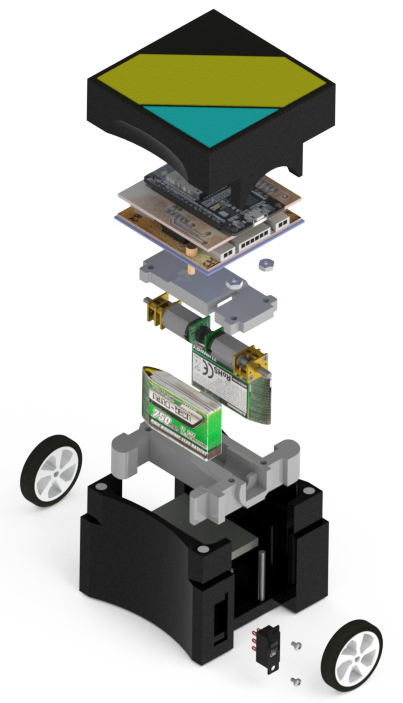
\includegraphics[width=0.5\textwidth]{figuras/robo/robo_completo_explodido.png}
    \caption{Vista explodida do robô completo.}
    \label{fig:robo_completo_explodido}
    \fonte{Própria.}
\end{figure}

\begin{figure}[H]
    \centering
    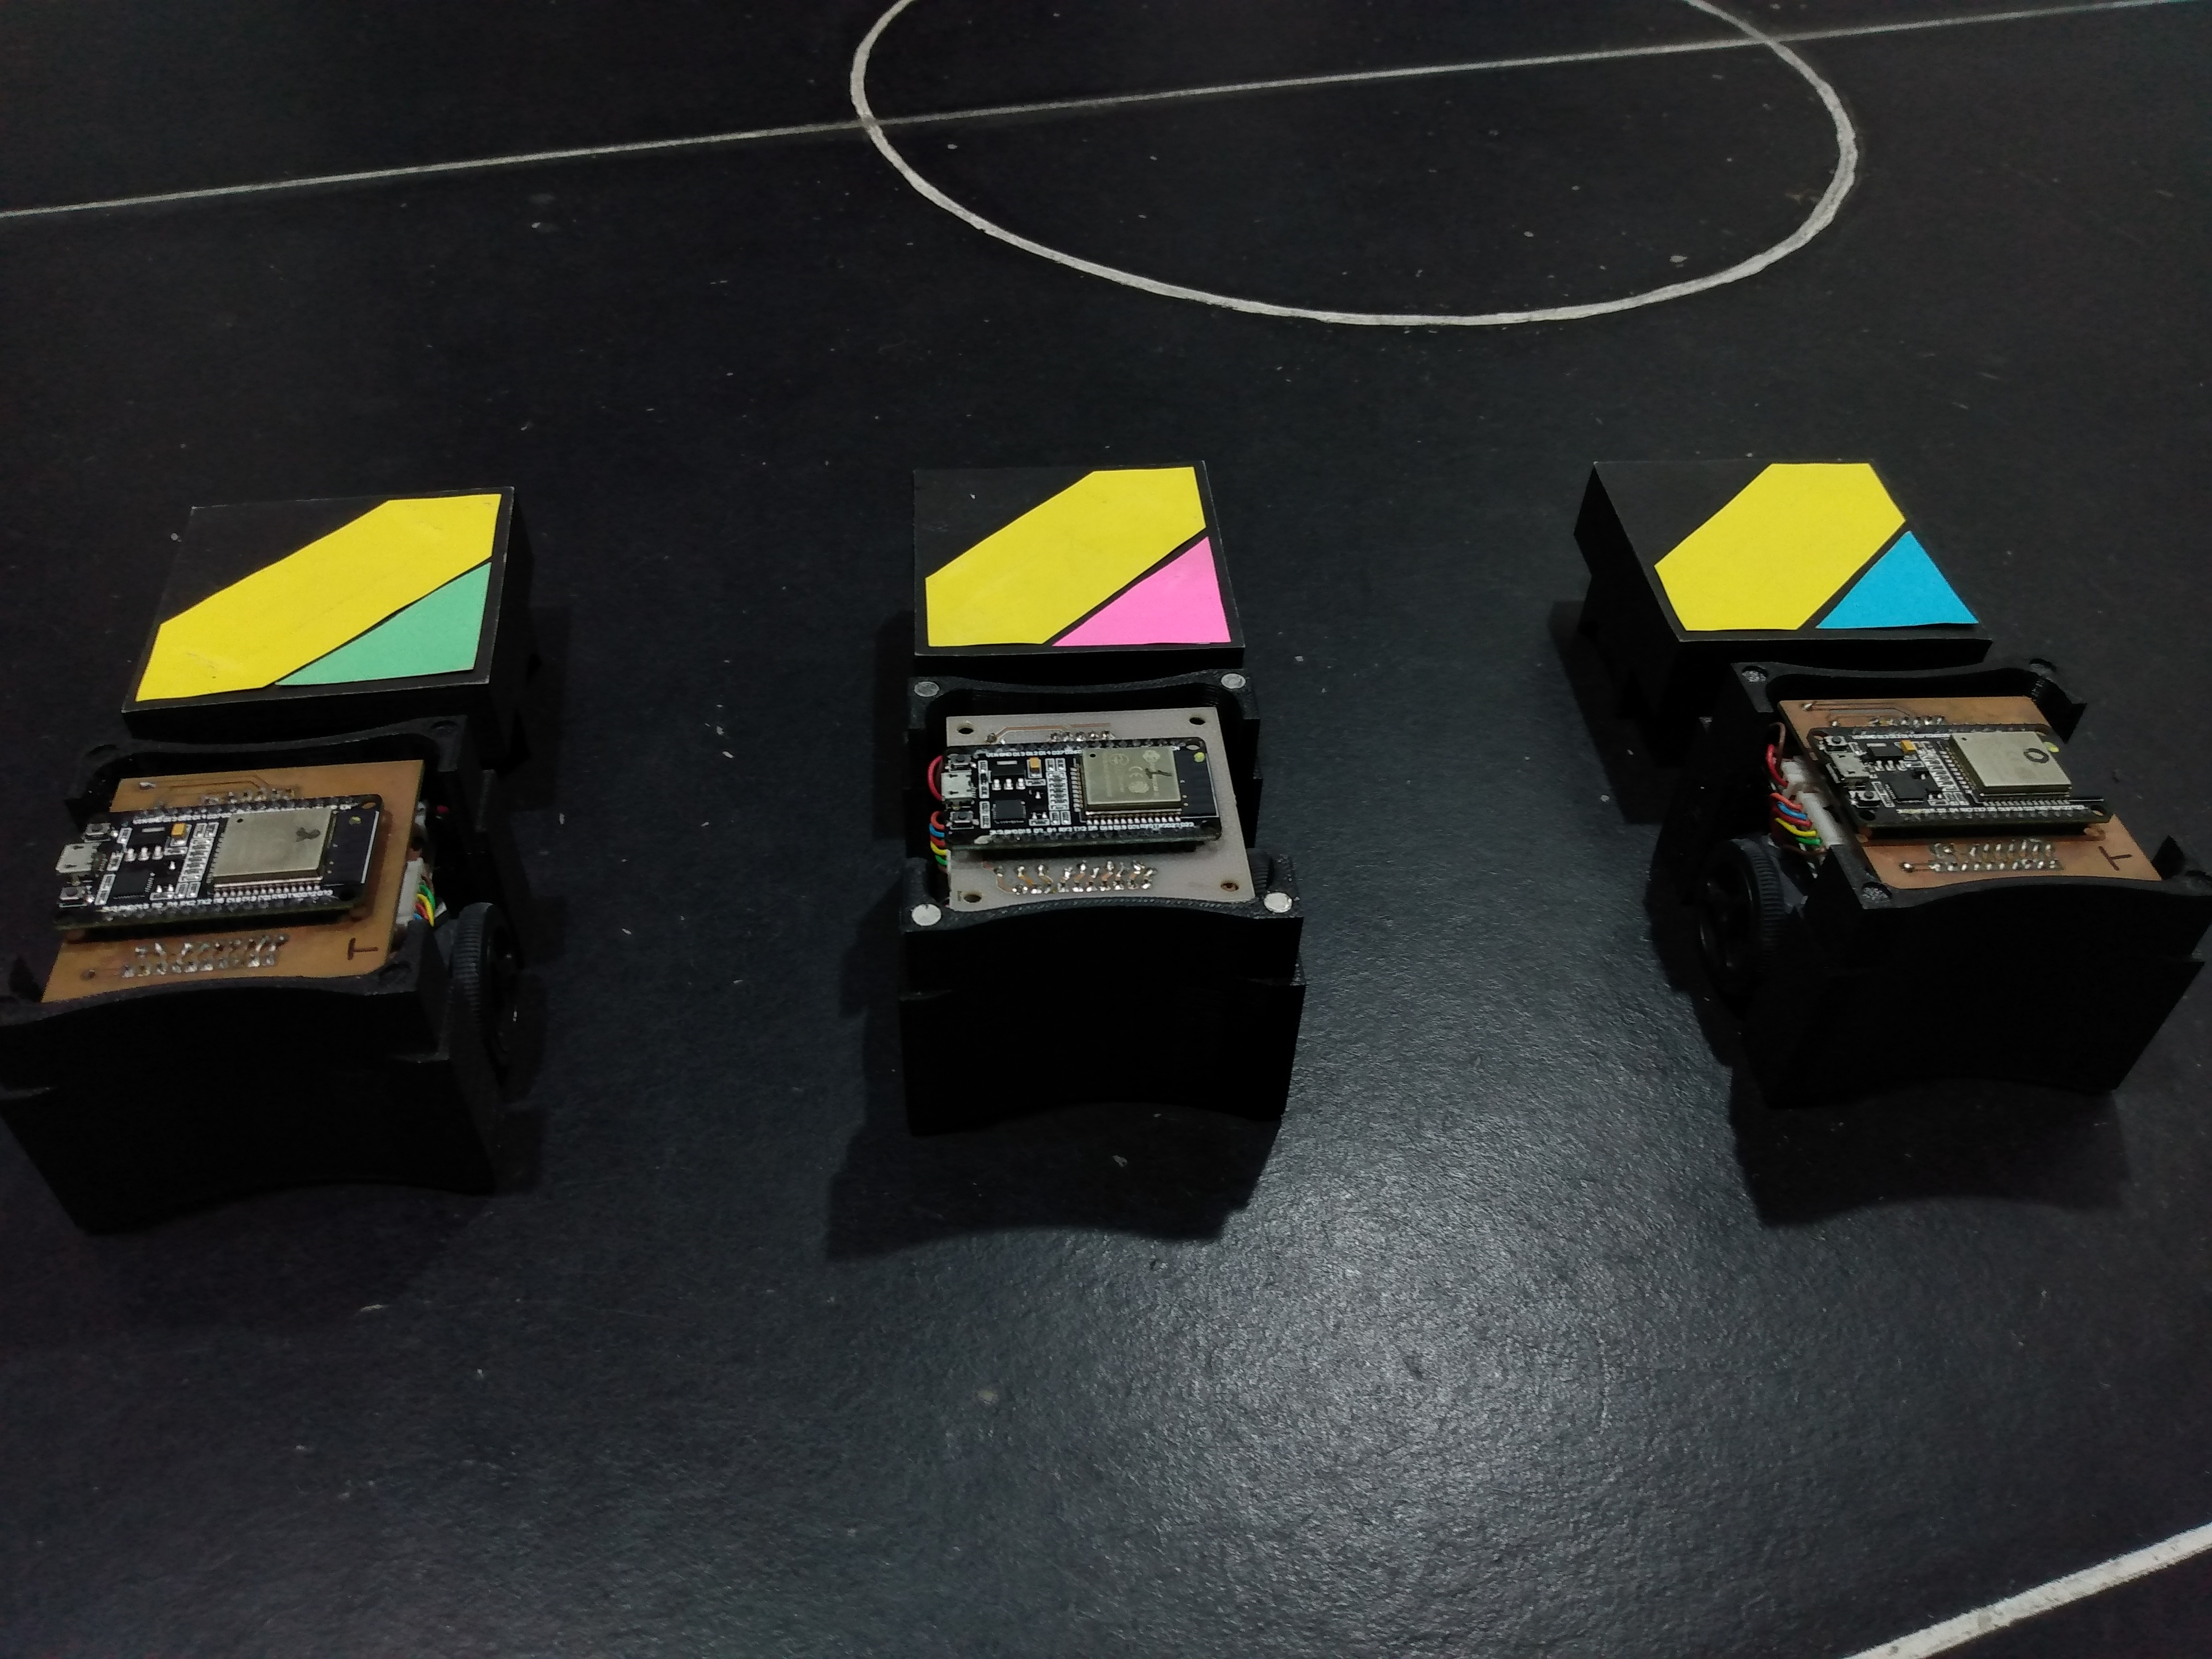
\includegraphics[width=0.5\textwidth]{textuais/robo/robos_capa_aberta.jpg}
    \caption{Frota de mini robôs da Equipe Poti de Futebol de robôs.}
    \label{fig:robos_capa_aberta}
    \fonte{Própria.}
\end{figure}

Já a Figura \ref{fig:robos_capa_aberta} mostra três dos robôs reais (um time) utilizados no laboratório.

As subseções seguintes apresentam mais detalhes a respeito do projeto desses robôs.
\subsection{Componentes}
% Motor: 
% https://www.pololu.com/product/2212
% https://www.pololu.com/product/2212
% Encoder:
% https://www.pololu.com/product/3081
% Driver motor:
% https://www.pololu.com/product/713
% ESP32:

São quatro o número de componentes básicos que compõem os robôs presentes neste trabalho, sendo eles: um par de atuadores (motor direito e esquerdo), um par de sensores de rotação (\textit{Encoder}s magnéticos), um driver motor multicanal, um microcontrolador e bateria recarregável. Devido as características dos componentes escolhidos para o projeto, apenas estes quatro tipos foram suficiente para compor a eletrônica do robô de forma a respeitar as restrições dimensionais, realizar o controle feedforward/backward de forma eficiência e com um bom período de amostragem e baixo gasto energético, além de um baixo custo financeiro.

A seguir serão apresentados mais detalhes dos componentes supracitados.

% 30:1 Micro Metal Gearmotor HP 6V with Extended Motor Shaft
\begin{figure}[H]
    \centering
    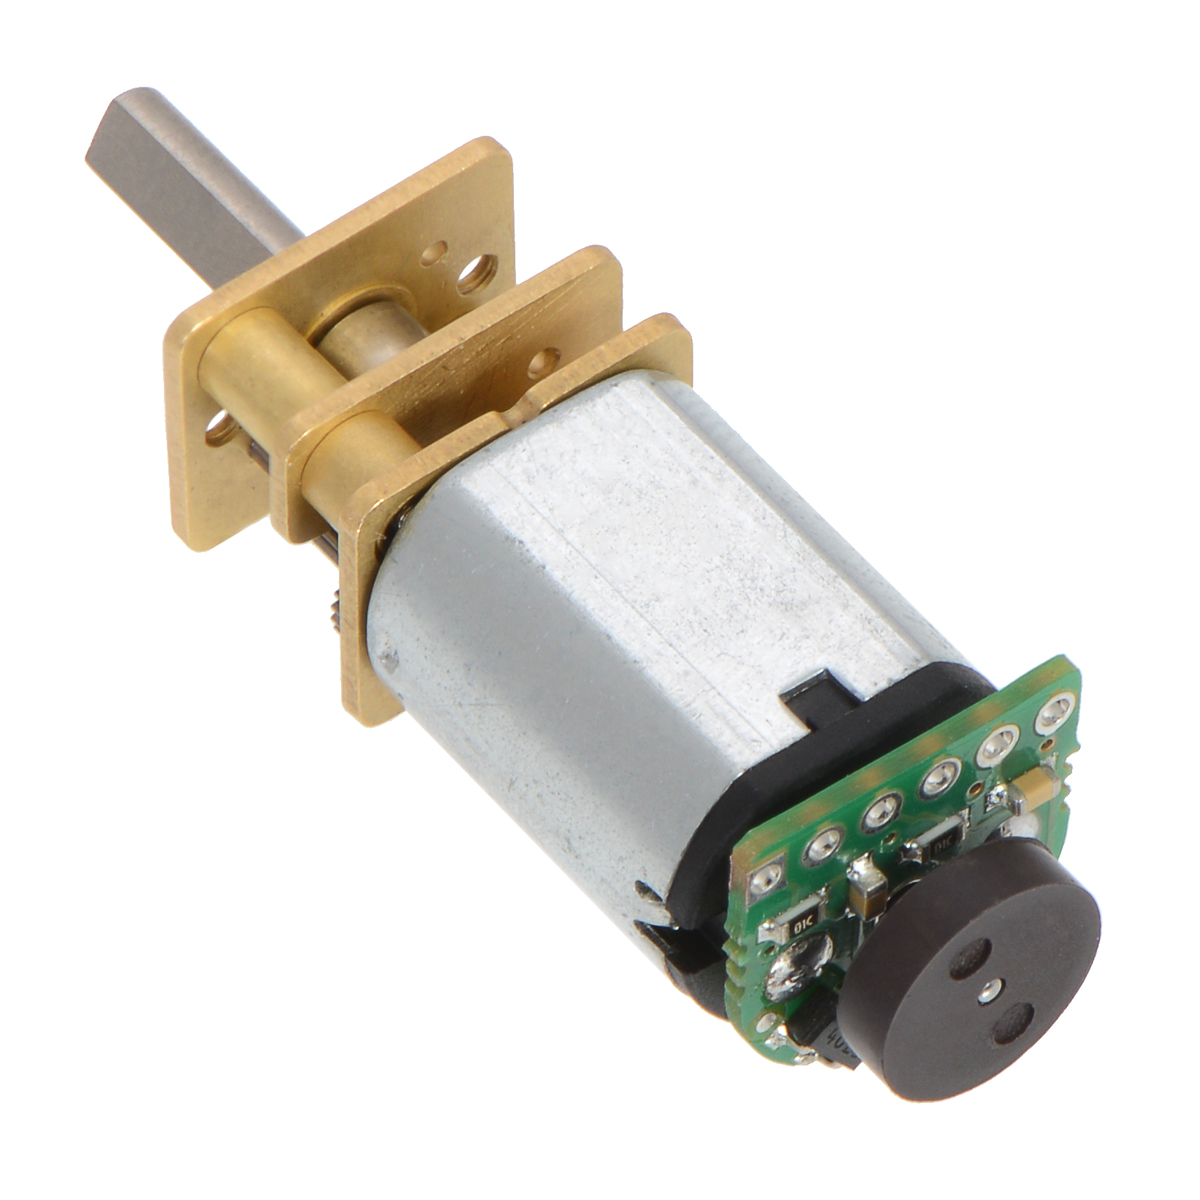
\includegraphics[width=3cm]{figuras/eletronica/motor_com_encoder.jpg}
    \caption{Micro Motor de 6V com caixa de redução de 30:1 e \textit{Encoder} magnético.}
    \label{fig:motor_com_encoder}
\end{figure}

A figura \ref{fig:motor_com_encoder} mostra o motor escolhido já com o \textit{Encoder} magnético colocado em seu eixo estendido (placa de circuito impresso com um Imã natural em forma de disco), esse é um micro motor de $6$V com uma caixa de redução de $\approx 30:1$ da \textit{Pololu}[?].

\begin{figure}[H]
    \centering
    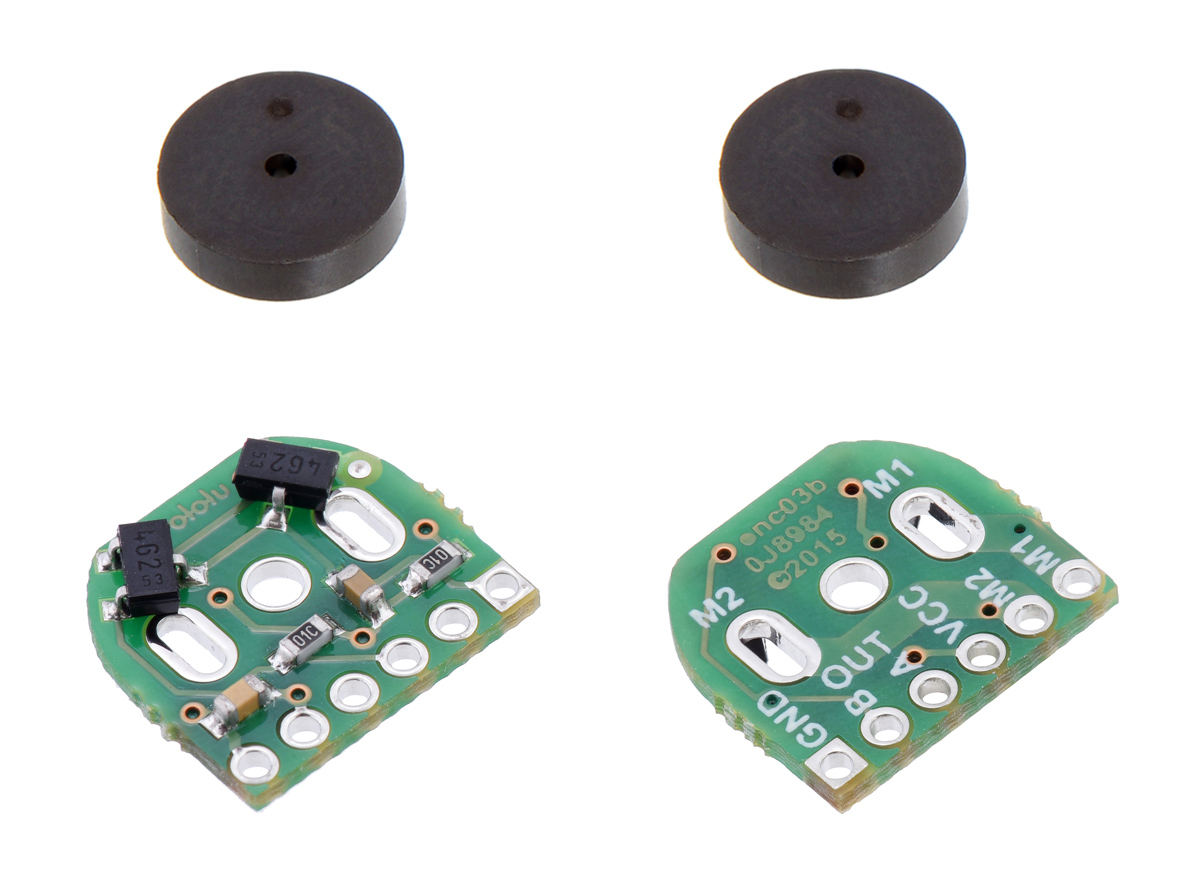
\includegraphics[width=5cm]{figuras/eletronica/encoder_frente_verso.jpg}
    \caption{Par de Encoders Magnéticos de $12$ pulsos por revolução ($12$CPR)}
    \label{fig:encoder}
\end{figure}

\begin{figure}[H]
    \centering
    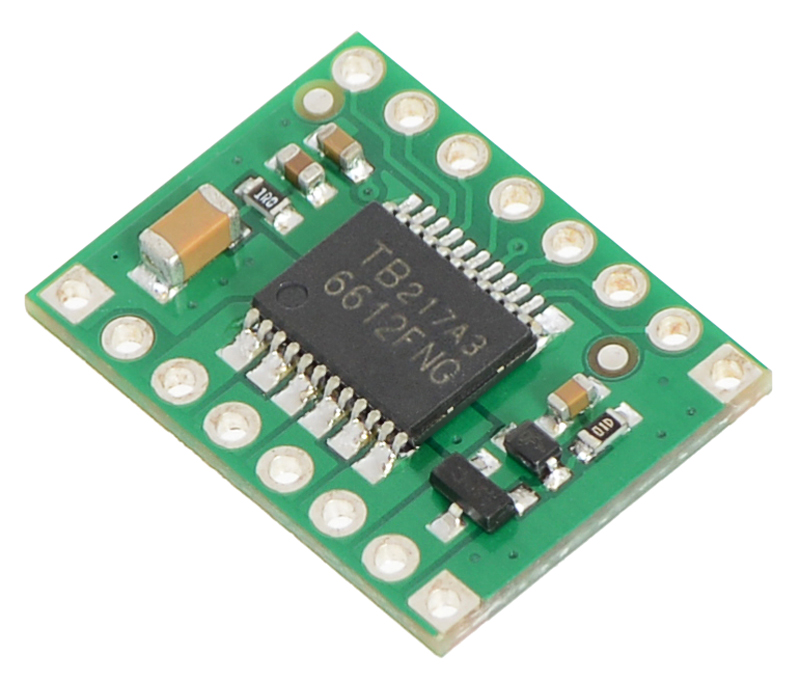
\includegraphics[width=3cm]{figuras/eletronica/driver.jpg}
    \caption{\textit{Driver} Motor TB6612FNG.}
    \label{fig:driver_motor}
\end{figure}

\begin{figure}[H]
    \centering
    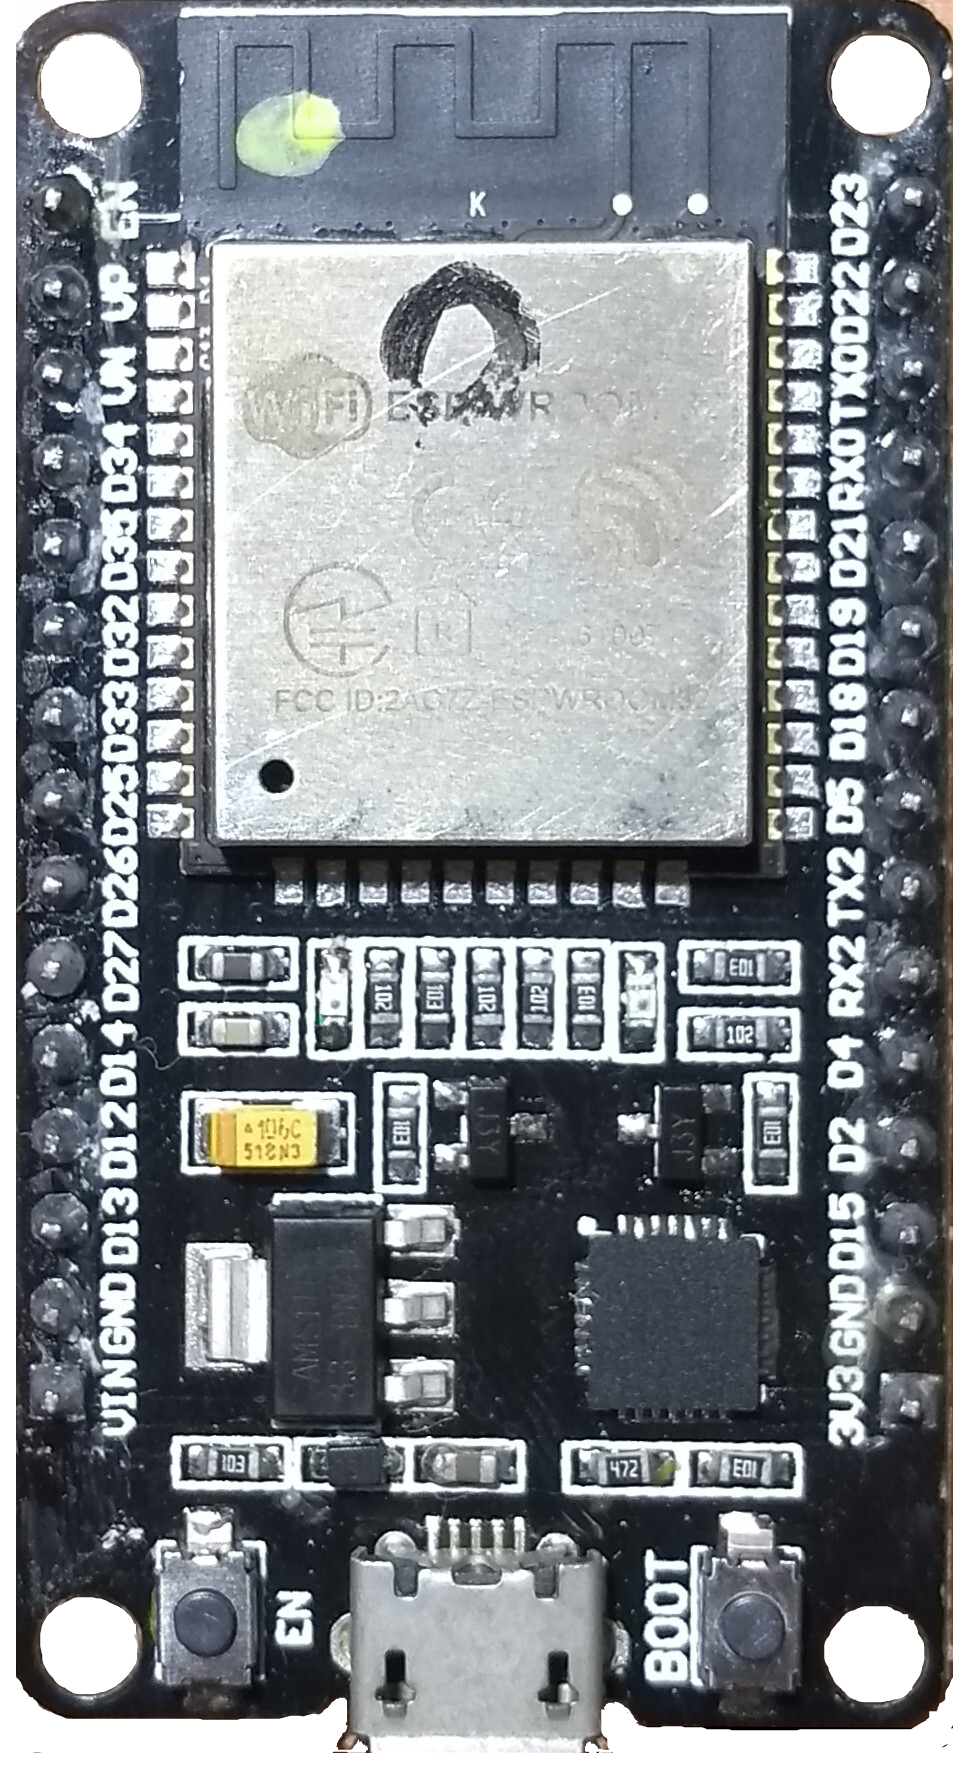
\includegraphics[width=3cm]{figuras/eletronica/esp32_kit.png}
    \caption{Placa de desenvolvimento ESP32 Dev1.}
    \fonte{Própria}
    \label{fig:esp32_kit}
\end{figure}
\subsection{Projeto Eletrônico}
% CIRCUITO ELÉTRICO/ELETRÔNICO COMPLETO
% MOSTRAR/EXPLICAR: PLACA DE CIRCUITO IMPRESSO DESENVOLVIDA
% TODO:
% ref:  https://produza.ind.br/gestao/pre-requisitos-tecnicos-para-montar-um-projeto-eletronico/

% \begin{figure}[H]
%     \centering
%     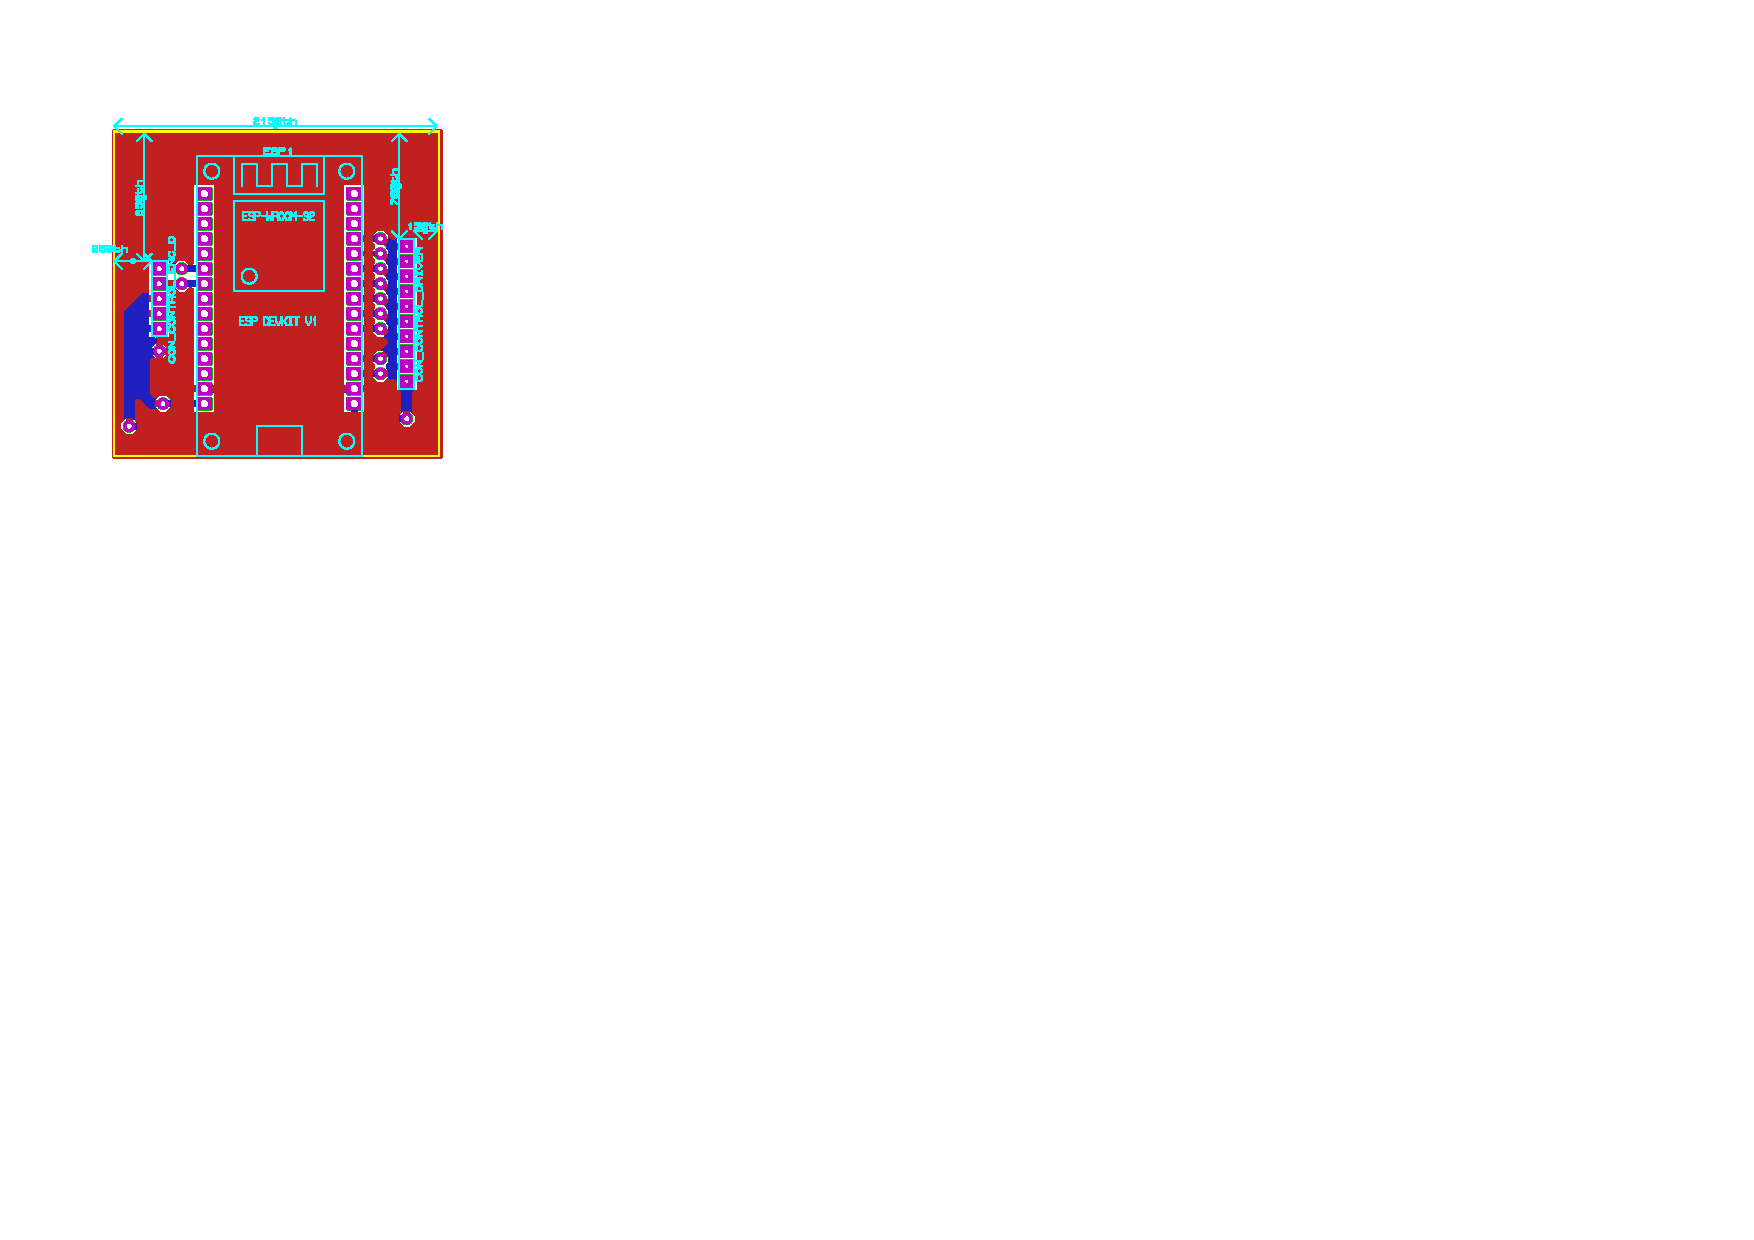
\includegraphics[width=\textwidth]{imagens/eletronica/placa/placa_controle_completa.pdf}
%     \caption{Caption}
%     % \label{fig:my_label}
% \end{figure}

% \begin{figure}[H]
%     \centering
%     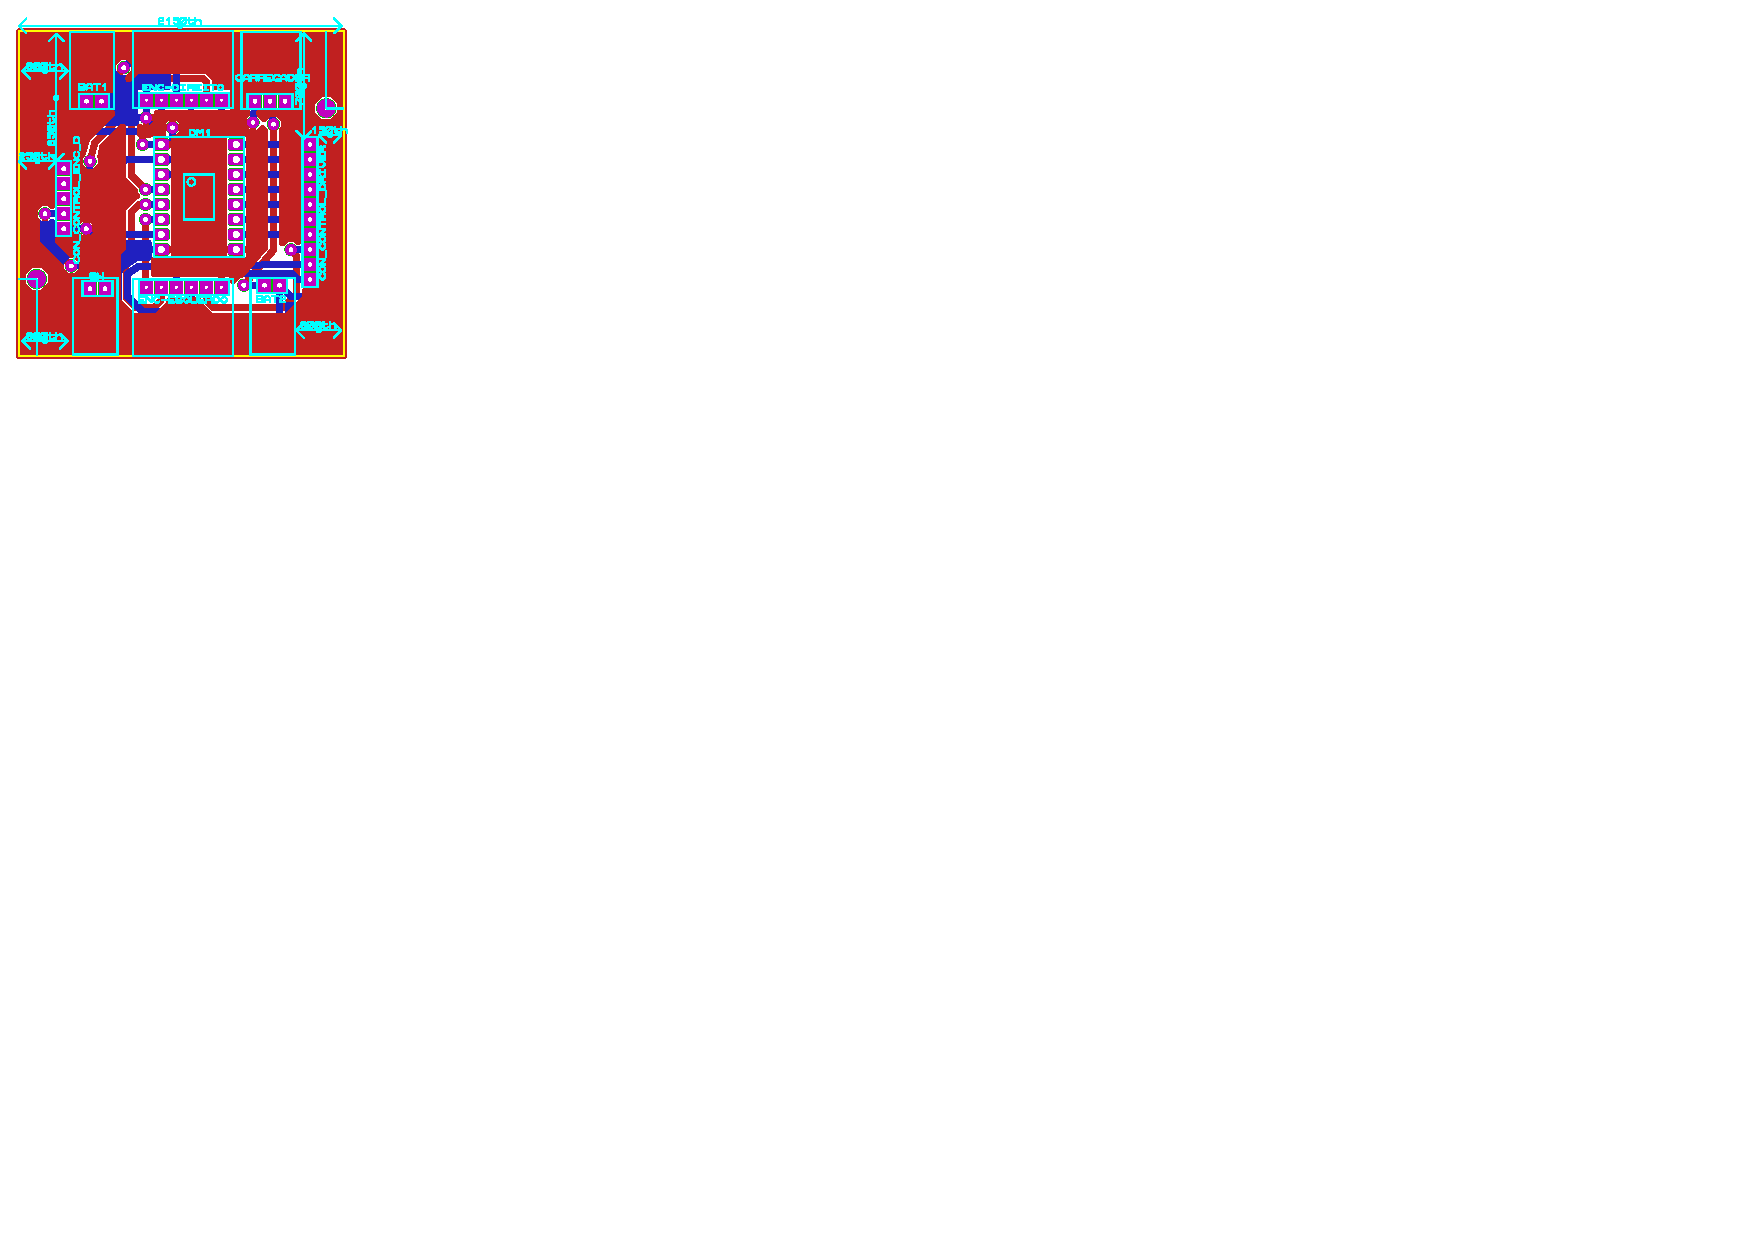
\includegraphics[width=\textwidth]{imagens/eletronica/placa/placa_driver_completa.pdf}
%     \caption{Caption}
%     % \label{fig:my_label}
% \end{figure}

\begin{enumerate}
    \item \textbf{Concepção inicial}:
        O principal objetivo por trás de se fazer uma nova placa de circuito eletrônico é acomodar os componentes, respeitando os limites das dimensões estabelecidos pela competição na qual os robôs serão utilizados (caber dentro de um cubo de $75$ mm de aresta). A placa deve conter o microcontrolador, no seu kit de desenvolvimento, \textit{Driver motor} para acionamento dos motores DCs, os \textit{Encoders} e ser alimentada por duas baterias de $1$ célula do tipo \textit{Lipo}.
        
    \item \textbf{Elaboração dos esquemáticos eletrônicos}:
        O esquemático foi a parte mais simples, pois não houve grandes mudanças nessa parte, com relação aos projetos de anos anteriores. A maior mudança foi o microcontrolador, que provocou dificuldades maiores na etapa seguinte, a elaboração do \textit{Layout}, devido às dimensões dos componentes.
        
        % inserir imagem do esquemático geral aqui
        
        \begin{figure}[H]
            \centering
            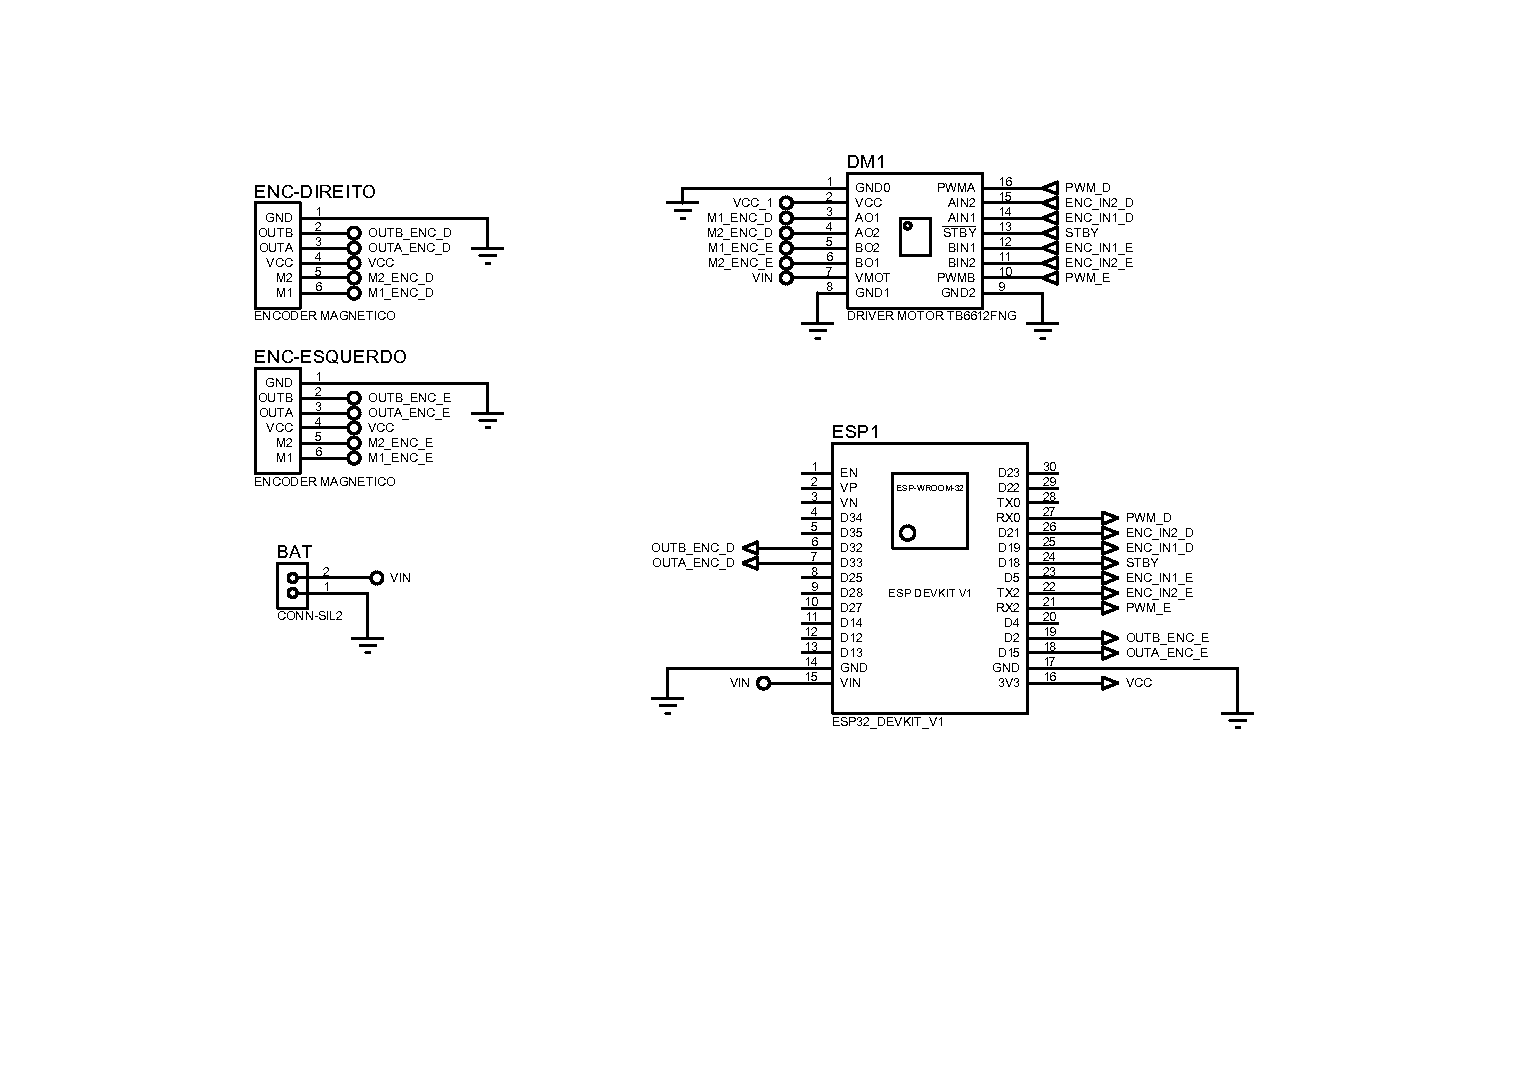
\includegraphics[width=\textwidth]{figuras/eletronica/placa/esquematico_completo.pdf}
            \caption{Esquemático.}
        \end{figure}
        
    \item \textbf{Elaboração do layout}:
        % inserir imagem do layout final aqui
        Este ponto foi o mais crítico nessa tarefa, devido à restrição de tamanho da placa ser de um quadrado com até $55$mm de lado. A solução adotada foi fazer em duas camadas, ou seja, duas placas cobreadas, ambas dupla face, dividindo os componentes. Em uma placa foi comportado o \textit{Driver}, bem como os conectores para os motores com os sensores e os conectores das baterias, e na outra apenas o microcontrolador. Para a conexão entre as placas foi utilizado um conector do tipo \textit{Head}, um macho e uma fêmea. Dessa forma, as placas conseguiram respeitar o limite dimensional e comportar todos os componentes necessários.
    \item \textbf{Realização de testes}:
        % faltou imagem de testes aqui
        Foram realizados testes antes da concepção da PCI, em \textit{Protoboards} para conferir se o circuito está funcionando como esperado e após a confecção, para se verificar a qualidade da confecção das placas.
        
        Também foram realizados testes individuais nos componentes, principalmente nos sensores, com o uso de osciloscópios. Verificou-se o funcionamento correto dos \textit{Encoders} e também conferiu-se se a distância entre os sensores poderia estar gerando interferência um no outro. Os resultados desses testes foram que todos os \textit{encoders} utilizados estão em bom estado, ou seja, funcionando como esperado e a distância que eles ficarão ao serem acomodados na estrutura não causa interferência um no outro.
    \item \textbf{Verificação e validação}
        Após testes individuais, de cada componente, foram realizados testes com a montagem completa, ou seja, os robôs montados por completo com as PCIs, baterias, motores e sensores. A validação foi por meio de controle manual dos robôs e testes simples de leitura de \textit{Encoder}, pois nessa etapa o \textit{Firmware} ainda não havida sido implementado.
\end{enumerate}